\documentclass{article}
\usepackage{tikz}
\usetikzlibrary{shapes.geometric}

\begin{document}

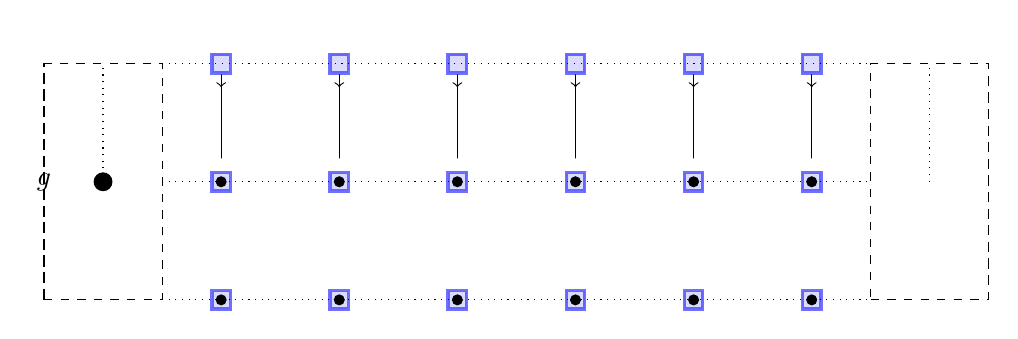
\begin{tikzpicture}[scale=1.5]
  % Define the style for the parallelepipeds
  \tikzstyle{parallelepiped} = [draw=blue!80, fill=blue!20, very thick, opacity=0.7]

  % Define the style for the points
  \tikzstyle{point} = [circle, fill=black, inner sep=0pt, minimum size=4pt]

  % Draw the parallelepipeds
  \foreach \x in {0, 1, 2, 3, 4, 5} {
    \node[parallelepiped] at (\x, 0) {};
    \node[parallelepiped] at (\x, 1) {};
    \node[parallelepiped] at (\x, -1) {};
  }

  % Draw the points
  \foreach \y in {0, -1} {
    \foreach \x in {0, 1, 2, 3, 4, 5} {
      \node[point] at (\x, \y) {};
    }
  }

  % Draw the horizontal lines
  \draw[dotted] (-0.5, 0) -- (5.5, 0);
  \draw[dotted] (-0.5, -1) -- (5.5, -1);
  \draw[dotted] (-0.5, 1) -- (5.5, 1);

  % Draw the vertical line for the special point "g"
  \draw[dotted] (-1, 0) -- (-1, 1);

  % Draw the special point "g"
  \node[point, draw, thick, circle, minimum size=6pt] at (-1, 0) {};

  % Label the special point "g"
  \node at (-1.5, 0) {$g$};

  % Draw the curved arrows
  \draw[->] (0, 0.3) .. controls +(-90:0.5) and +(90:0.5) .. (0, 0.8);
  \draw[->] (1, 0.3) .. controls +(-90:0.5) and +(90:0.5) .. (1, 0.8);
  \draw[->] (2, 0.3) .. controls +(-90:0.5) and +(90:0.5) .. (2, 0.8);
  \draw[->] (3, 0.3) .. controls +(-90:0.5) and +(90:0.5) .. (3, 0.8);
  \draw[->] (4, 0.3) .. controls +(-90:0.5) and +(90:0.5) .. (4, 0.8);
  \draw[->] (5, 0.3) .. controls +(-90:0.5) and +(90:0.5) .. (5, 0.8);

  % Draw the dashed parallelepipeds for the layers
  \foreach \x in{-1, 6} {
    \draw[dashed] (\x-1/2, -1) -- (\x+1/2, -1) -- (\x+1/2, 1) -- (\x-1/2, 1) -- cycle;
  }
  
  % Draw the dashed lines for the layers
  \draw[dashed] (-1.5, -1) -- (-1.5, 1);
  \draw[dashed] (6.5, -1) -- (6.5, 1);
  \draw[dotted] (6, 0) -- (6, 1);
\end{tikzpicture}

\end{document}